\documentclass[final]{lmuposter}
% helpful for justifying the boxes, use the following in the header:
%
\setlength{\parindent}{0pt}

% German language
\usepackage[ngerman]{babel}
% Fonts of package UTF8
\usepackage[utf8x]{inputenc}

% pgf and tikz for graphics
\usepackage{pgf}
\usepackage{pgflibrarysnakes}
\usepackage{tikz}

% mathematical symbols of the ams package
\usepackage{amsmath}
\usepackage{amssymb}
\usepackage{bbm}

% supfigures
\usepackage{subfig}

% macros for vectors, matrix and so on
\newsavebox{\fmbox}
\newenvironment{fmpage}[1]
	{\begin{lrbox}{\fmbox}\begin{minipage}{#1}}
	{\end{minipage}\end{lrbox}\fbox{\usebox{\fmbox}}}
%
% Puts a algorithm environment
\newenvironment{algorithm}[1][]{%
	\begin{table}[h]
	\centering
	\begin{minipage}[t]{12cm}
	\hspace{\stretch{2}} {\caption{\label{#1} #1}}
	\rule[1.5ex]{12cm}{0.01cm}\\
	%\hspace{\stretch{2}} {\tiny \textsc{ #1}}}
	\hspace{\stretch{2}} \\
	% SPACE BEFORE \\ IS IMPORTANT, ELSE NO STRETCHING
	\vspace{-4ex}
	\begin{list}{#1}{\labelwidth=12em \leftmargin=120pt}
	\vspace{-1ex}
}{%
	\end{list}
	\rule[1ex]{12cm}{0.01cm}\\
	\end{minipage}
	\vspace{-2ex}
	\end{table}
}
%
\newcommand{\atem}[2]{\item[\texttt{#1}] #2\vspace{1ex}}
%
% Some math stuff, you need to include \usepackage{amsmath} 
%
%
%\mathop is needed to  get the spacing correct,
%
\newcommand{\sign}{\mathop{\mathrm{sign}}}
%
% greek symbols are displayed fat, too 
%
\renewcommand{\vector}[1]{\boldsymbol{#1}}
%
% use straight letters for matrixes
%
\renewcommand{\matrix}[1]{\mathbf{#1}}
%
% Some further definitions
%
\newcommand{\set}[1]{\mathbb{#1}}
\newcommand{\transpose}{\mathsf{T}}
\newcommand{\unity}{\mathbbm{1}}

\usepackage{MnSymbol}

% multicols package
\usepackage{multicol}

% Python source code highlighting. Uses the listings package. Use lstinputlistings in the boxes of the
% poster.
% Python listing setup
\usepackage{color}
\usepackage[procnames]{listings}
\usepackage{setspace}
\renewcommand{\lstlistlistingname}{Code Listings}
\renewcommand{\lstlistingname}{Code Listing}
\definecolor{gray}{gray}{0.5}
\definecolor{lightgray}{gray}{0.9}
\definecolor{green}{rgb}{0,0.5,0}
\definecolor{lightgreen}{rgb}{0,0.7,0}
\definecolor{orange}{rgb}{1,0.5,0}
\definecolor{purple}{rgb}{0.5,0,0.5}
\definecolor{darkred}{rgb}{0.5,0,0}


\lstset{
language=python,
extendedchars=true,
%basicstyle=\ttfamily\small\setstretch{1},
basicstyle=\footnotesize,
mathescape=true,
breaklines=true,
numbers=left,
numbersep=10pt,
numberstyle=\tiny,
framexleftmargin=30pt,
xleftmargin=55pt,
stringstyle=\color{green},
showstringspaces=false,
alsoletter={1234567890},
otherkeywords={\ , \}, \{},
keywordstyle=\color{blue},
emph={access,and,as,break,class,continue,def,del,elif,else,%
except,exec,finally,for,from,global,if,import,in,is,%
lambda,not,or,pass,print,raise,return,try,while,assert},
emphstyle=\color{orange}\bfseries,
emph={[2]self},
emphstyle=[2]\color{gray},
emph={[4]ArithmeticError,AssertionError,AttributeError,BaseException,%
DeprecationWarning,EOFError,Ellipsis,EnvironmentError,Exception,%
False,FloatingPointError,FutureWarning,GeneratorExit,IOError,%
ImportError,ImportWarning,IndentationError,IndexError,KeyError,%
KeyboardInterrupt,LookupError,MemoryError,NameError,None,%
NotImplemented,NotImplementedError,OSError,OverflowError,%
PendingDeprecationWarning,ReferenceError,RuntimeError,RuntimeWarning,%
StandardError,StopIteration,SyntaxError,SyntaxWarning,SystemError,%
SystemExit,TabError,True,TypeError,UnboundLocalError,UnicodeDecodeError,%
UnicodeEncodeError,UnicodeError,UnicodeTranslateError,UnicodeWarning,%
UserWarning,ValueError,Warning,ZeroDivisionError,abs,all,any,apply,%
basestring,bool,buffer,callable,chr,classmethod,cmp,coerce,compile,%
complex,copyright,credits,delattr,dict,dir,divmod,enumerate,eval,%
execfile,exit,file,filter,float,frozenset,getattr,globals,hasattr,%
hash,help,hex,id,input,int,intern,isinstance,issubclass,iter,len,%
license,list,locals,long,map,max,min,object,oct,open,ord,pow,property,%
quit,range,raw_input,reduce,reload,repr,reversed,round,set,setattr,%
slice,sorted,staticmethod,str,sum,super,tuple,type,unichr,unicode,%
vars,xrange,zip},
emphstyle=[4]\color{purple}\bfseries,
morecomment=[s][\color{lightgreen}]{"""}{"""},
morekeywords={and,as,assert,break,class,continue,def,del,elif,else,except,
     finally,for,from,global,if,import,in,is,lambda,not,or,pass,print,
     return,try,while,with,yield},
commentstyle=\color{red}\slshape,
%literate={>>>}{\textbf{\textcolor{darkred}{>{>}>}}}3%
%         {...}{{\textcolor{gray}{...}}}3,
procnamekeys={def,class},
procnamestyle=\color{blue}\textbf,
%framexleftmargin=0mm, framextopmargin=0mm, frame=ovalbox,
backgroundcolor=\color{lightgray},
frame=single,
framerule=0pt,
}



% Bibliography.
\usepackage[numbers,sort&compress, square]{natbib}
%
% Remove the bibliography header.
%
\makeatletter
\renewenvironment{thebibliography}[1]{%
%     \section*{\refname}%
%      \@mkboth{\MakeUppercase\refname}{\MakeUppercase\refname}%
      \list{\@biblabel{\@arabic\c@enumiv}}%
           {\settowidth\labelwidth{\@biblabel{#1}}%
            \leftmargin\labelwidth
            \advance\leftmargin\labelsep
            \@openbib@code
            \usecounter{enumiv}%
            \let\p@enumiv\@empty
            \renewcommand\theenumiv{\@arabic\c@enumiv}}%
      \sloppy
      \clubpenalty4000
      \@clubpenalty \clubpenalty
      \widowpenalty4000%
      \sfcode`\.\@m}
     {\def\@noitemerr
       {\@latex@warning{Empty `thebibliography' environment}}%
      \endlist}
\makeatother

% some modifications for the lists environment
%\renewcommand{\labelitemii}{$\blacktriangleright$}%
\setlength{\itemsep}{1mm}
\setlength{\parsep}{1mm}

\begin{document}
\nocite{obspy}
%\lstset{language=Python, showstringspaces=false, numbers=left, numberstyle=\tiny, basicstyle=\small}
%
% Document header
%
\PosterHead{\textbf{\LARGE ObsPy: A Python toolbox for seismology}\\[0.4ex] \textit{\Large interaktive Anwendung und schnelle Prototypenentwicklung} \\[0.5ex]
\large \underline{Lion Krischer}$^{\text{a}}$, Moritz Beyreuther$^{\text{a}}$, Robert Barsch$^{\text{a}}$, Tobias Megies$^{\text{a}}$, Yannik Behr$^{\text{b}}$, Joachim Wassermann$^{\text{a}}$\\ $^{\text{a}}$ LMU München \hspace{2em}  $^{\text{b}}$ Victoria University of Wellington, New Zealand\\
Department für Geo- und Umweltwissenschaften (Geophysik),
Ludwig-Maximilians-Universität München\\
Kontakt: \textit{krischer@geophysik.uni-muenchen.de}, \textbf{http://www.obspy.org}}

%
%\renewcommand{\capsize}{\footnotesize}
%
\setlength{\columnsep}{\MyBoxHSep}
\vspace{-1.5em}
\begin{multicols}{2}

%
% First box.
%
\MyBox[8em]{
\section*{1~~~Abstract}
\textbf{Python} ermöglicht es, die Vorteile einer ausgewachsenen Programmiersprache mit der Flexibilität einer interaktiven Skriptsprache zu verbinden. Die Standardbibliothek und die hohe Qualität von wissenschaftlichen Drittmodulen erlaubt eine schnelle Entwicklung von Programmen.

\textbf{ObsPy} erweitert Python um Import- und Exportroutinen für Wellenformdatenformate und Metadaten und enthält häufig benötigte Routinen für diverse Aufgabenfelder in der Seismologie.

Es steht zudem die breite Palette an Funktionalität von numerischen Modulen zur Matrizenprogrammierung wie \textbf{NumPy} (http://numpy.scipy.org) oder \textbf{SciPy} (http://scipy.org) zur Verfügung. Zusammen mit z.B. \textbf{IPython} und \textbf{Matplotlib} stellt ObsPy eine mächtige, textbasierte, leicht erlernbare, interaktive Umgebung dar, die komplett aus freien Softwarepaketen besteht und leicht erweiterbar ist.

ObsPy ist \textbf{modular} aufgebaut, mit dem Ziel die Abhängigkeiten zu minimieren und steht unter der \textbf{GPL/LGPLv3} als Open Source Software zur Verfügung.
}\vspace{\MyBoxVSep}

%
% Second box.
%
\MyBox[8em]{
\section*{2~~~Eine kurze Einführung in Python}
% Include code.
\lstinputlisting[firstline=2]{code/python_example.py}
Der Einrückungsgrad markiert zusammengehörige Codeblöcke. (siehe \textit{for}-Schleife)
}\vspace{\MyBoxVSep}

%
% Third box.
%
\MyBox[8em]{
\section*{3~~~Lesen und Schreiben}
ObsPy erweitert Python um \textbf{Import- und Exportroutinen} für \textbf{MiniSEED, GSE2, SAC, SEISAN und die Seismic Handler Formate Q und ASCII}.

Hierbei werden sämtliche Daten in einem Stream Objekt gespeichert.
% Include code.
\lstinputlisting[firstline=1, lastline=5]{code/reading.py}
Einfaches Auslesen multiplexer Datenströme: Jede Spur wird in einem eigenen Trace Objekt innerhalb des Stream Objekts gespeichert. Jeder Trace hat ein Stats Objekt, das die Metainformationen enthält. Die Daten selbst sind als \textbf{numpy.ndarrays} vorhanden und können somit mit den mächtigen Routinen von NumPy und SciPy weiterverarbeitet werden.
Die Stream und Trace Objekte haben diverse Methoden, z.B. die plot() Methode des Stream Objekts:
\lstinputlisting[firstline=7, lastline=7, firstnumber=6]{code/reading.py}

\begin{center}
\begin{tikzpicture}
\node[above right,text width=0.9\textwidth]at(0cm,0cm){ 
\tiny
\centering
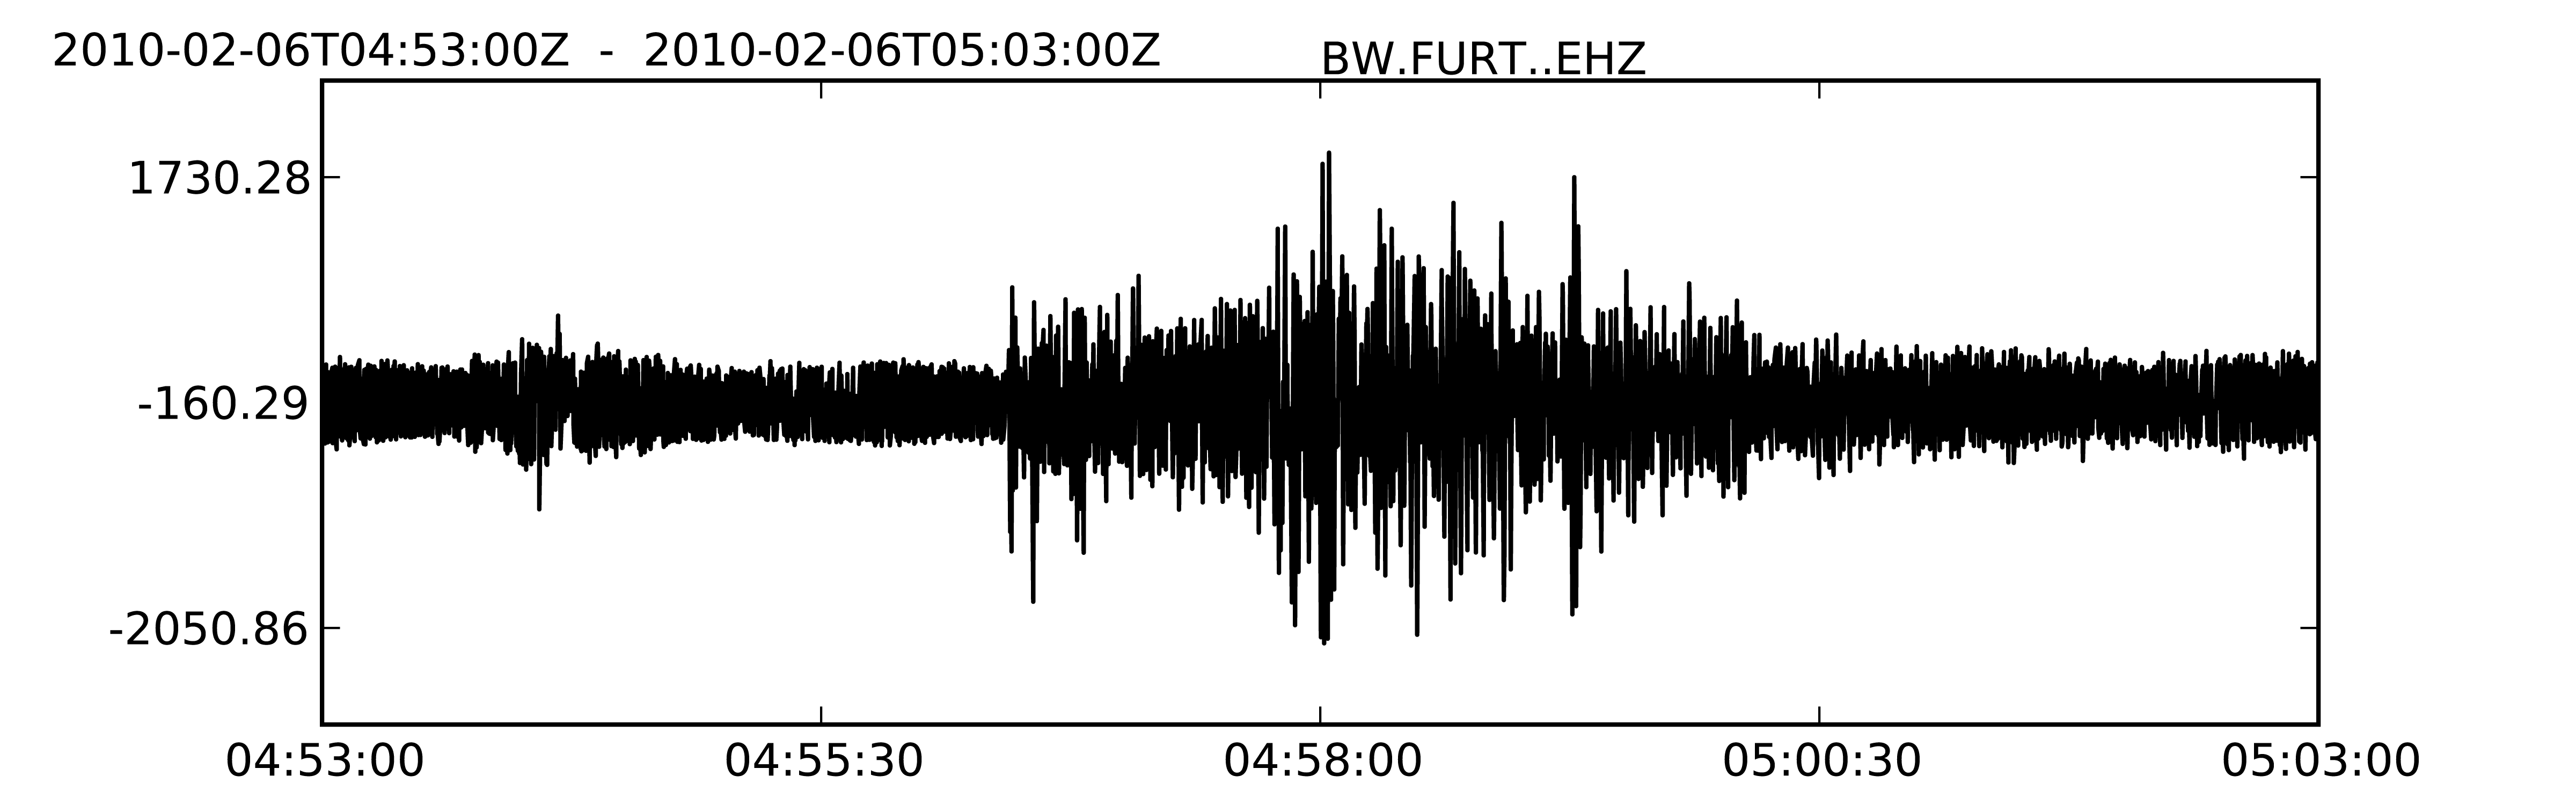
\includegraphics[width=0.9\textwidth]{simple_plot}\\[-3ex]
};
\end{tikzpicture}
{\newline \small \textbf{Abbildung~1}: Grafische Darstellung des Stream Objekts. Erstellt mit obspy.imaging.
} \\[.5\MyBoxVSep]
\end{center}

\vspace{2ex}
Geschrieben werden die Daten mit der write() Methode.
\lstinputlisting[firstline=9, lastline=9, firstnumber=7]{code/reading.py}


}\vspace{\MyBoxVSep}

\MyBox[8em]{
\section*{4~~~SEED/XML-SEED Unterstützung}
XML-SEED \citep{xseed} ist eine XML-Repräsentation des Dataless-SEED Formats \citep{seed}. ObsPy erlaubt die Verlustfreie Konvertierung zwischen beiden Formaten. So wird aus
\lstinputlisting{code/seed_example.py}
die folgende XML-Ausgabe
\lstinputlisting[firstline=2, lastline=5]{code/xseed_example.py}


}\vspace{\MyBoxVSep}

\columnbreak%\\
%
% Fourth box.
%

\MyBox[8em]{
\section*{6~~~obspy.signal (Instrumentenkorrektur)}
\begin{multicols}{2}
Dieses Beispiel zeigt die Korrektur eines STS2-Seismometers auf ein 1 Hz Instrument mit Hilfe von \textbf{obspy.signal}.
\newline
Die Daten werden mit \textbf{obspy.core} eingelesen und anschließend wird der Mittelwert abgezogen.
\lstinputlisting[firstline=8, lastline=8, firstnumber=8]{code/korrektur.py}
Jetzt werden die Daten mit Hilfe der seisSim() Funktion aus obspy.signal korrigiert. \textit{sts2} und \textit{onehzinst} sind Python Dictionaries, die Informationen zur den Intrumentenantworten enthalten.
\lstinputlisting[firstline=17, lastline=20, firstnumber=17]{code/korrektur.py}
\columnbreak
\begin{center}
\begin{tikzpicture}
\node[above right,text width=.45\MyBoxWidth]at(0cm,0cm){ 
\tiny
\centering
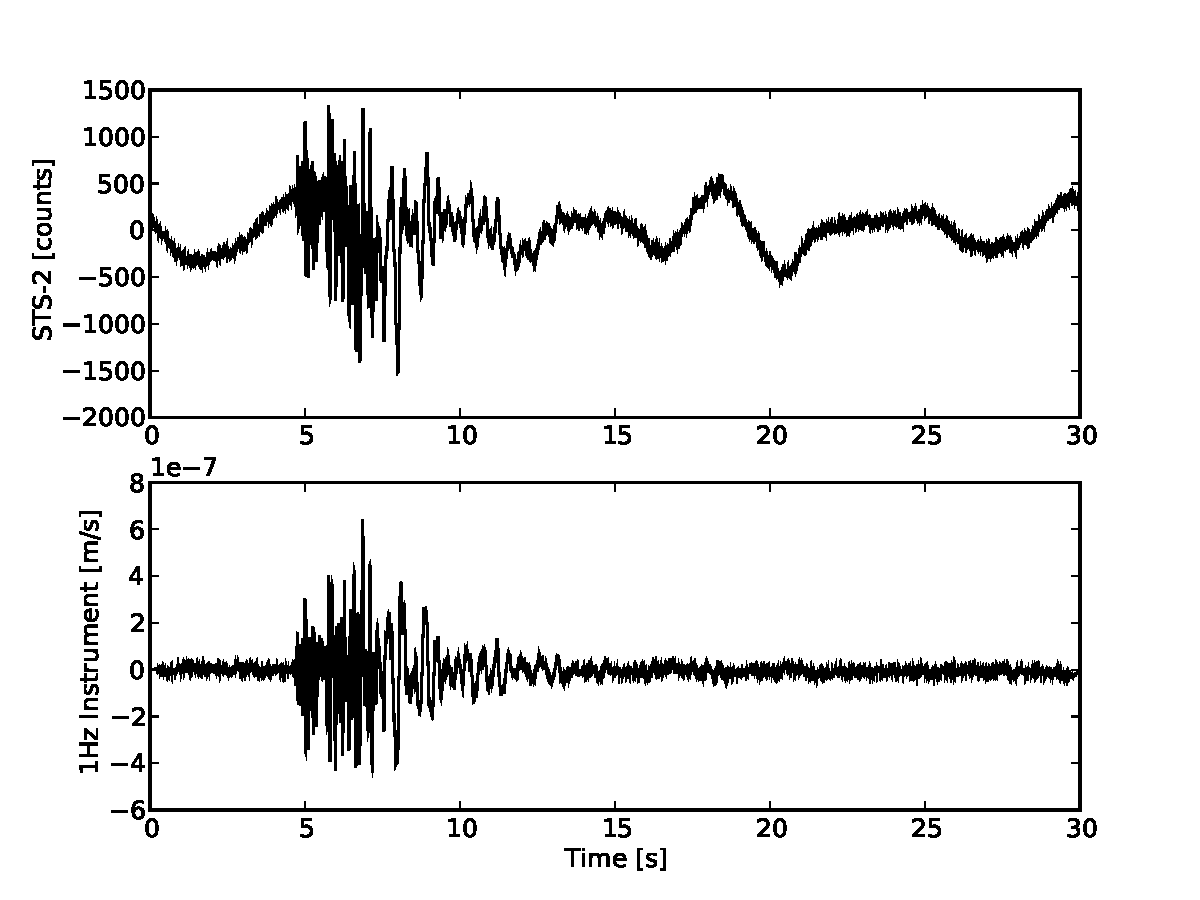
\includegraphics[height=.35\MyBoxWidth]{korrektur}\\[-3ex]
};
\end{tikzpicture}
	{\small
	\textbf{Abbildung~4}: Instrumtenkorrektur eines STS2 auf ein 1Hz Instrument.
	} \\[.5\MyBoxVSep]
\end{center}

\end{multicols}

}\vspace{\MyBoxVSep}
%
% Sixth box.
%



%
% Seventh box.
%

%
% Eigth box.
%
\MyBox[8em]{
\section*{7~~~obspy.imaging}
Das \textbf{obspy.imaging} Modul bietet Routinen zur grafischen Darstellung von Seismogrammen, Spektrogrammen und Herdflächenlösungen an.

\begin{multicols}{2}
\lstset{numbers=none}

\begin{center}
\begin{tikzpicture}
\node[above right,text width=.45\MyBoxWidth]at(0cm,0cm){ 
\tiny
\centering
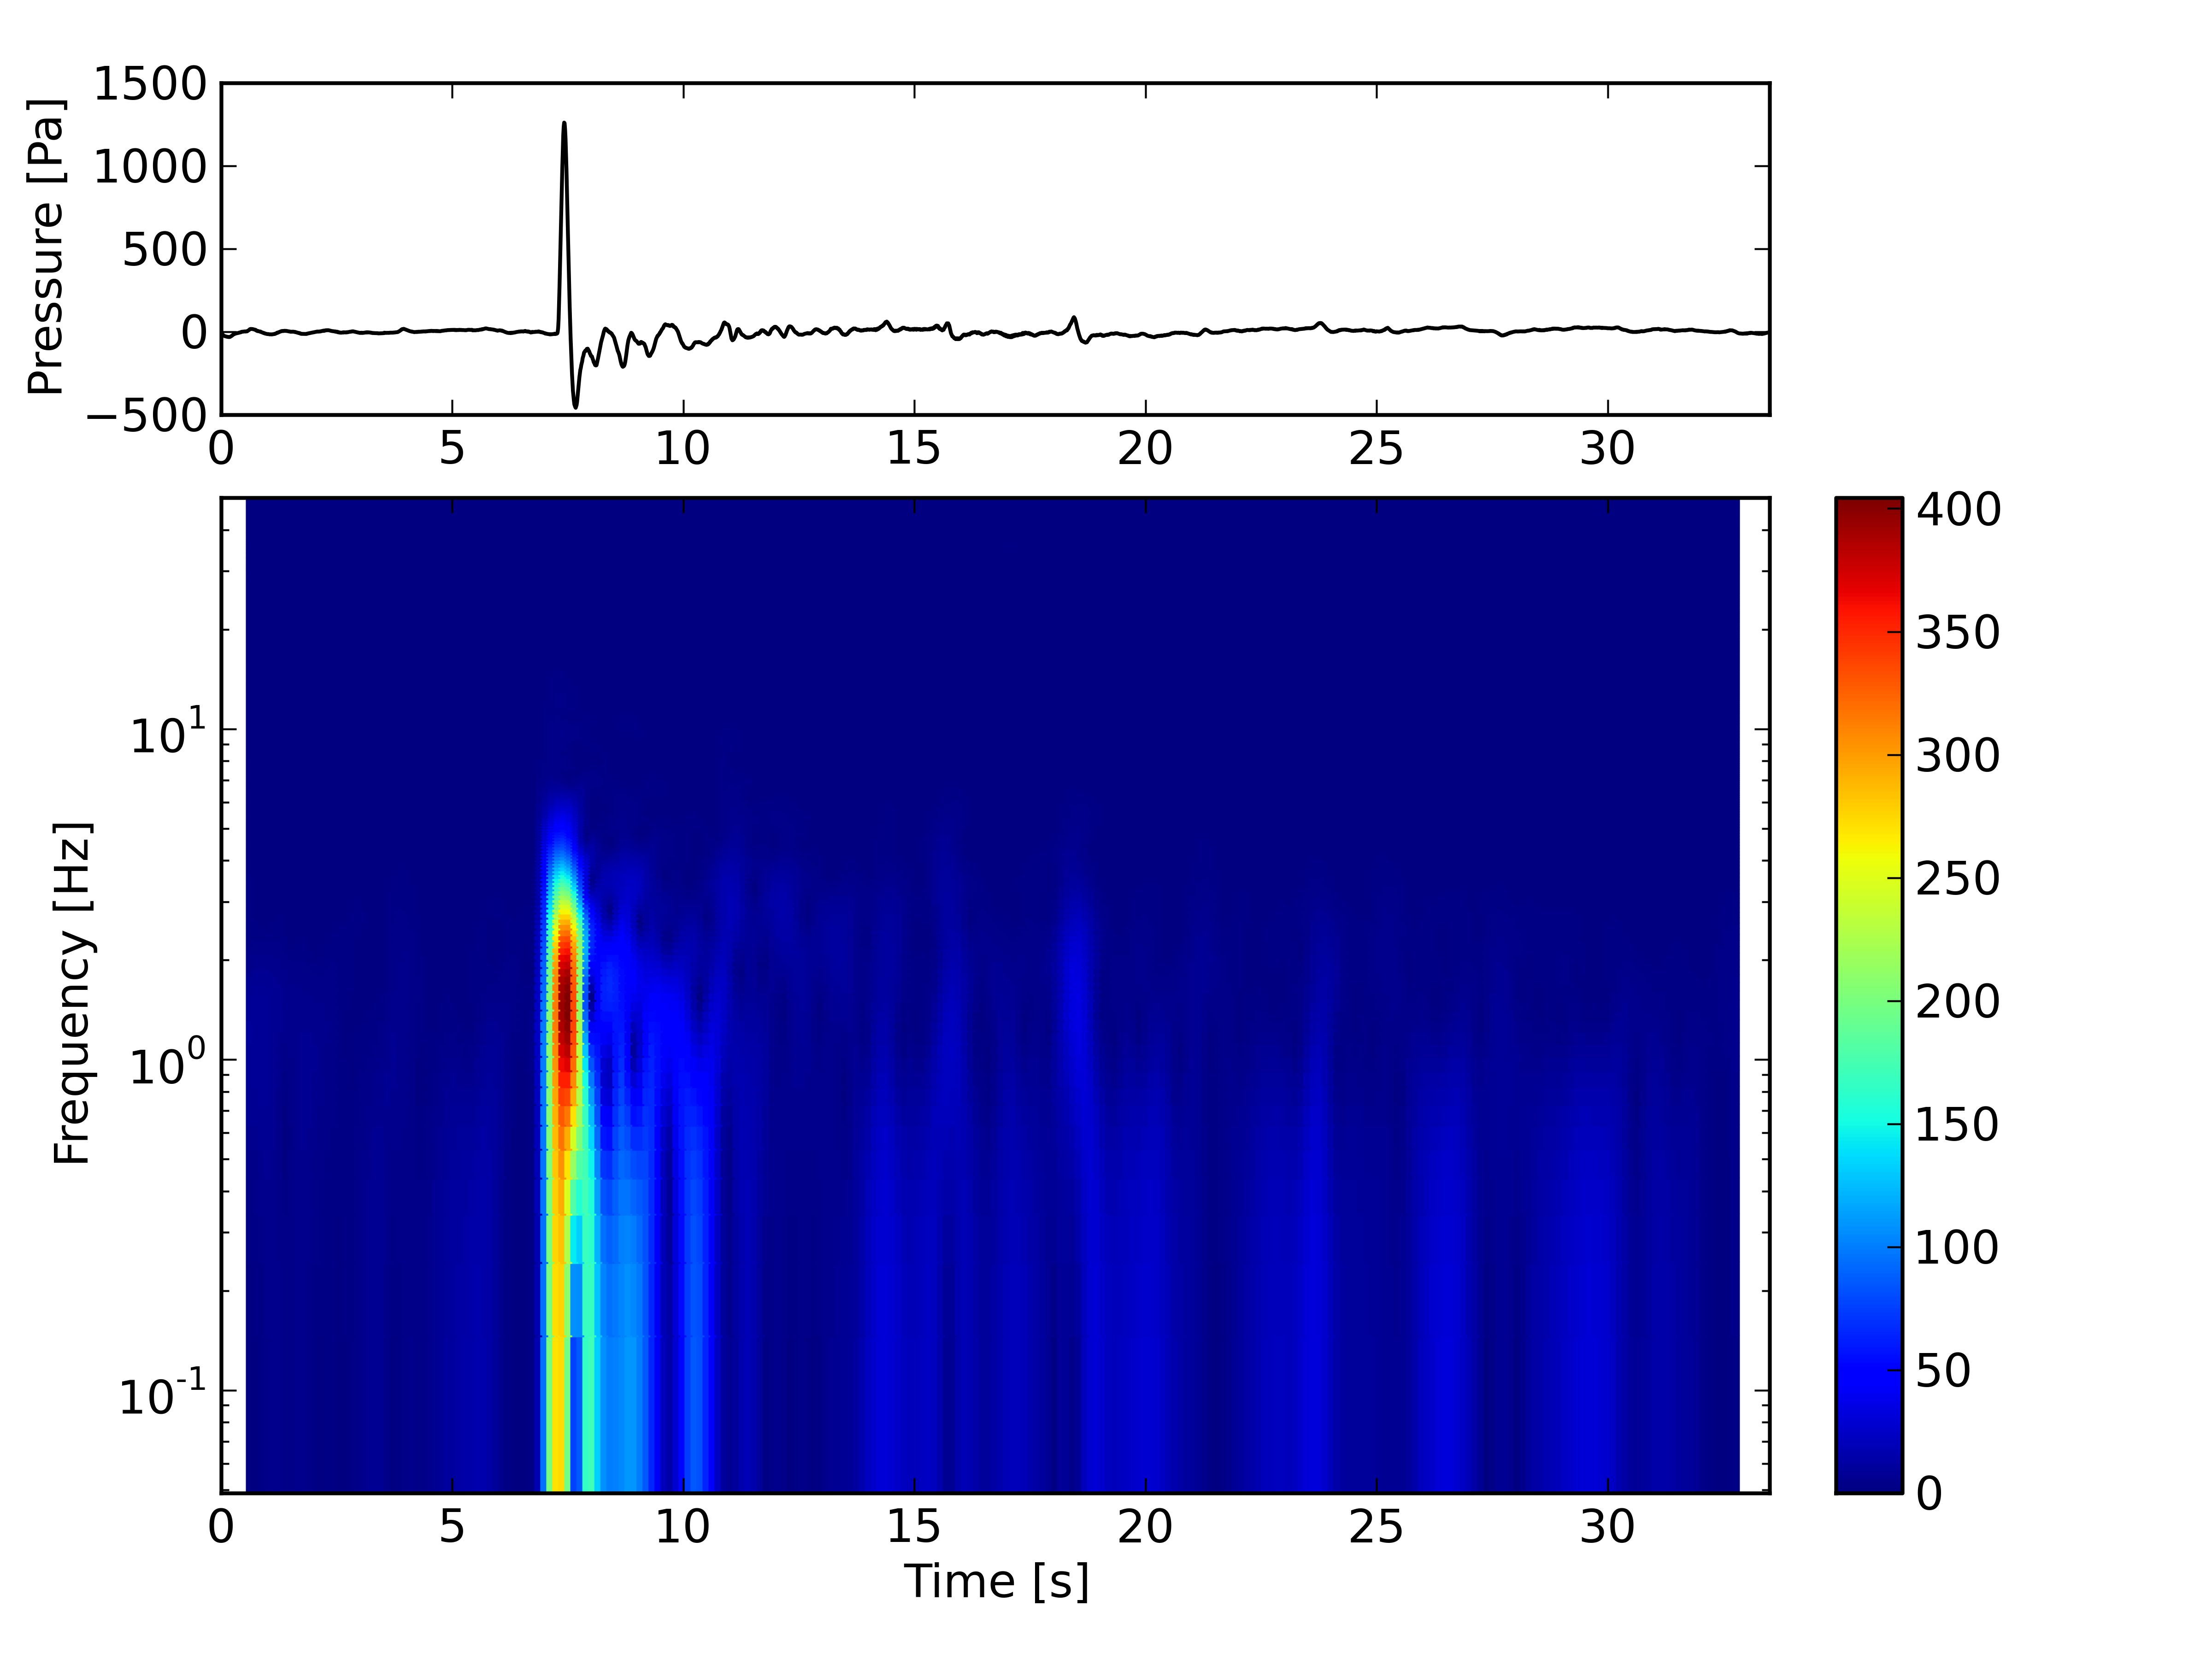
\includegraphics[height=.35\MyBoxWidth]{spectrogram_small}\\[-3ex]
};
\end{tikzpicture}
	{\small
	\textbf{Abbildung~2}: Spektrogramm, das mit Hilfe von obspy.imaging.spectrogram erstellt wurde.
	} \\[.5\MyBoxVSep]
\end{center}

\columnbreak
Herdflächenlösungen können als \textit{[Strike, Dip, Rake]} oder mit sechs unabhängigen Komponenten des Momententensors angeben werden.
\lstinputlisting[firstline=8, lastline= 11]{code/beachballs.py}
Jede Lösung wird in einen Graphen eingezeichnet.
\lstinputlisting[firstline=18, lastline=19, firstnumber=4]{code/beachballs.py}

\begin{center}
\begin{tikzpicture}
\node[above right,text width=.45\MyBoxWidth]at(0cm,0cm){ 
\tiny
\centering
%XXX: Replace with large pictures before printing!

\includegraphics[width=.45\MyBoxWidth]{beachball-collection.pdf}\\[-3ex]
};
\end{tikzpicture}
	{\small
	\textbf{Abbildung~3}: Eine Sammlung von Herdflächenlösungen, erstellt mit obspy.imaging.beachball.
	} \\[.5\MyBoxVSep]
\end{center}
\end{multicols}
\lstset{numbers=left}
%\begin{figure}
%  \centering
%  \subfloat[][]{\label{fig:gull}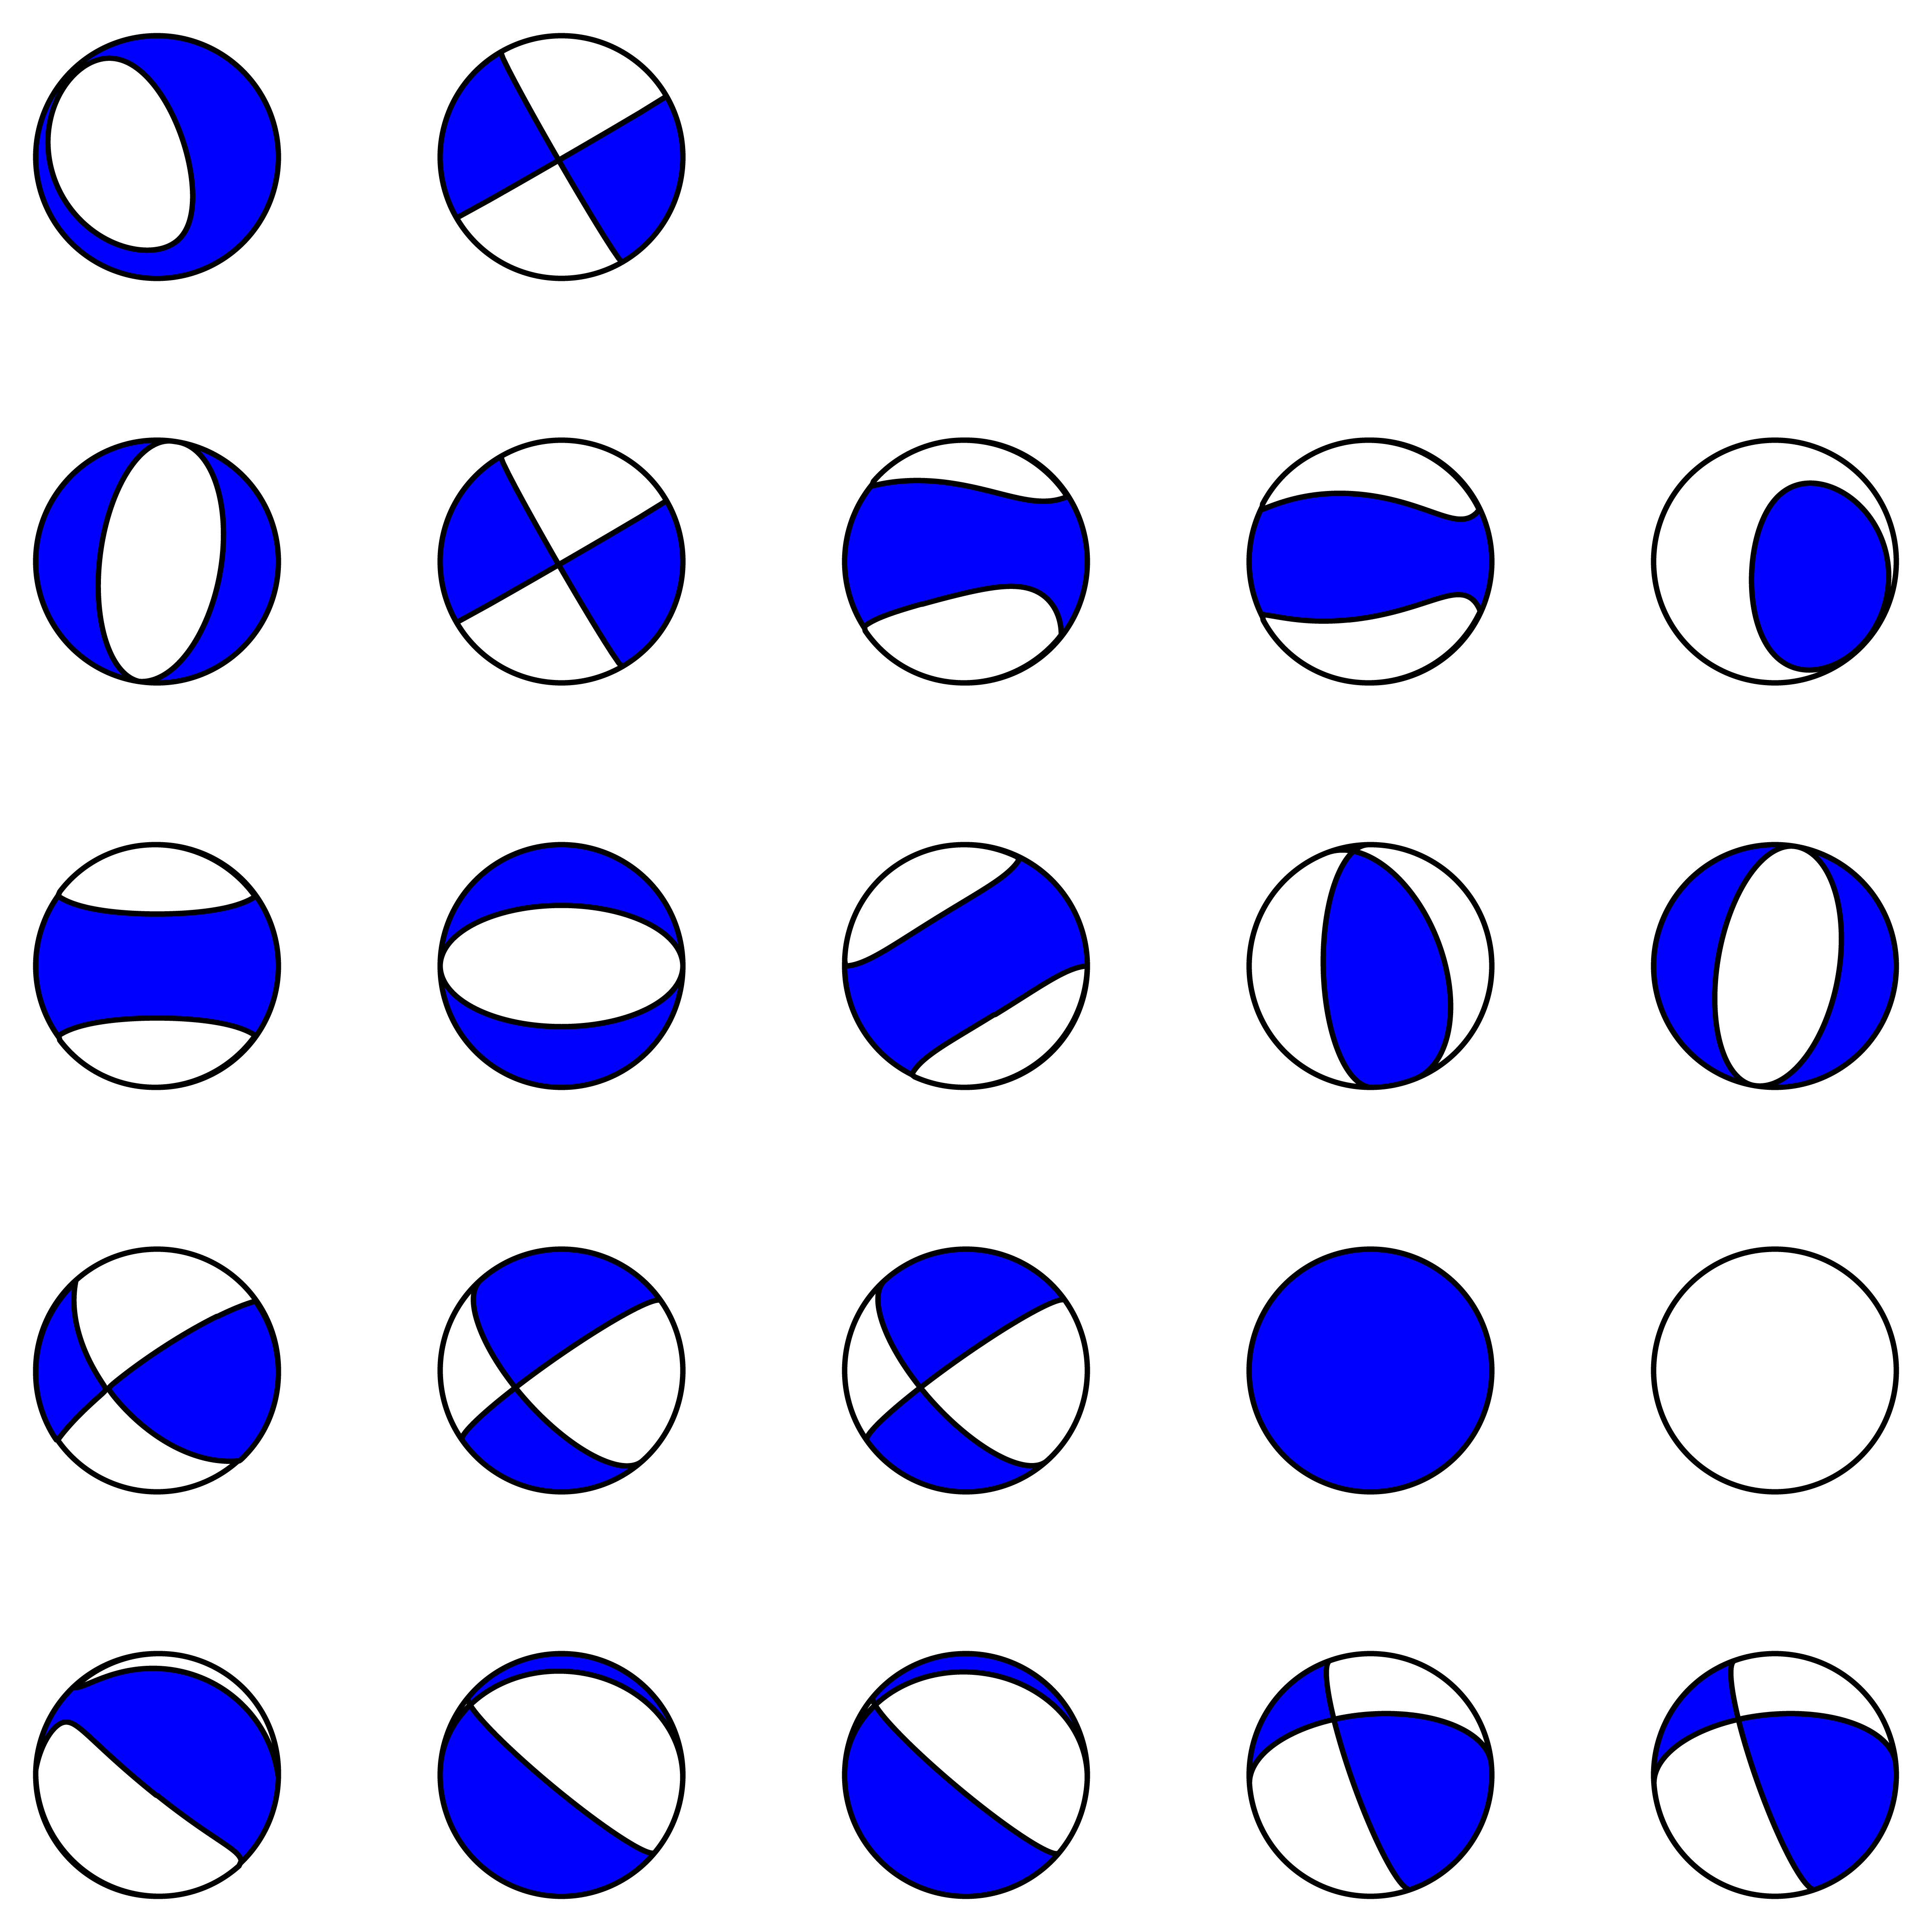
\includegraphics[width=0.45\textwidth]{beachballs}}                
%  \subfloat[][]{\label{fig:tiger}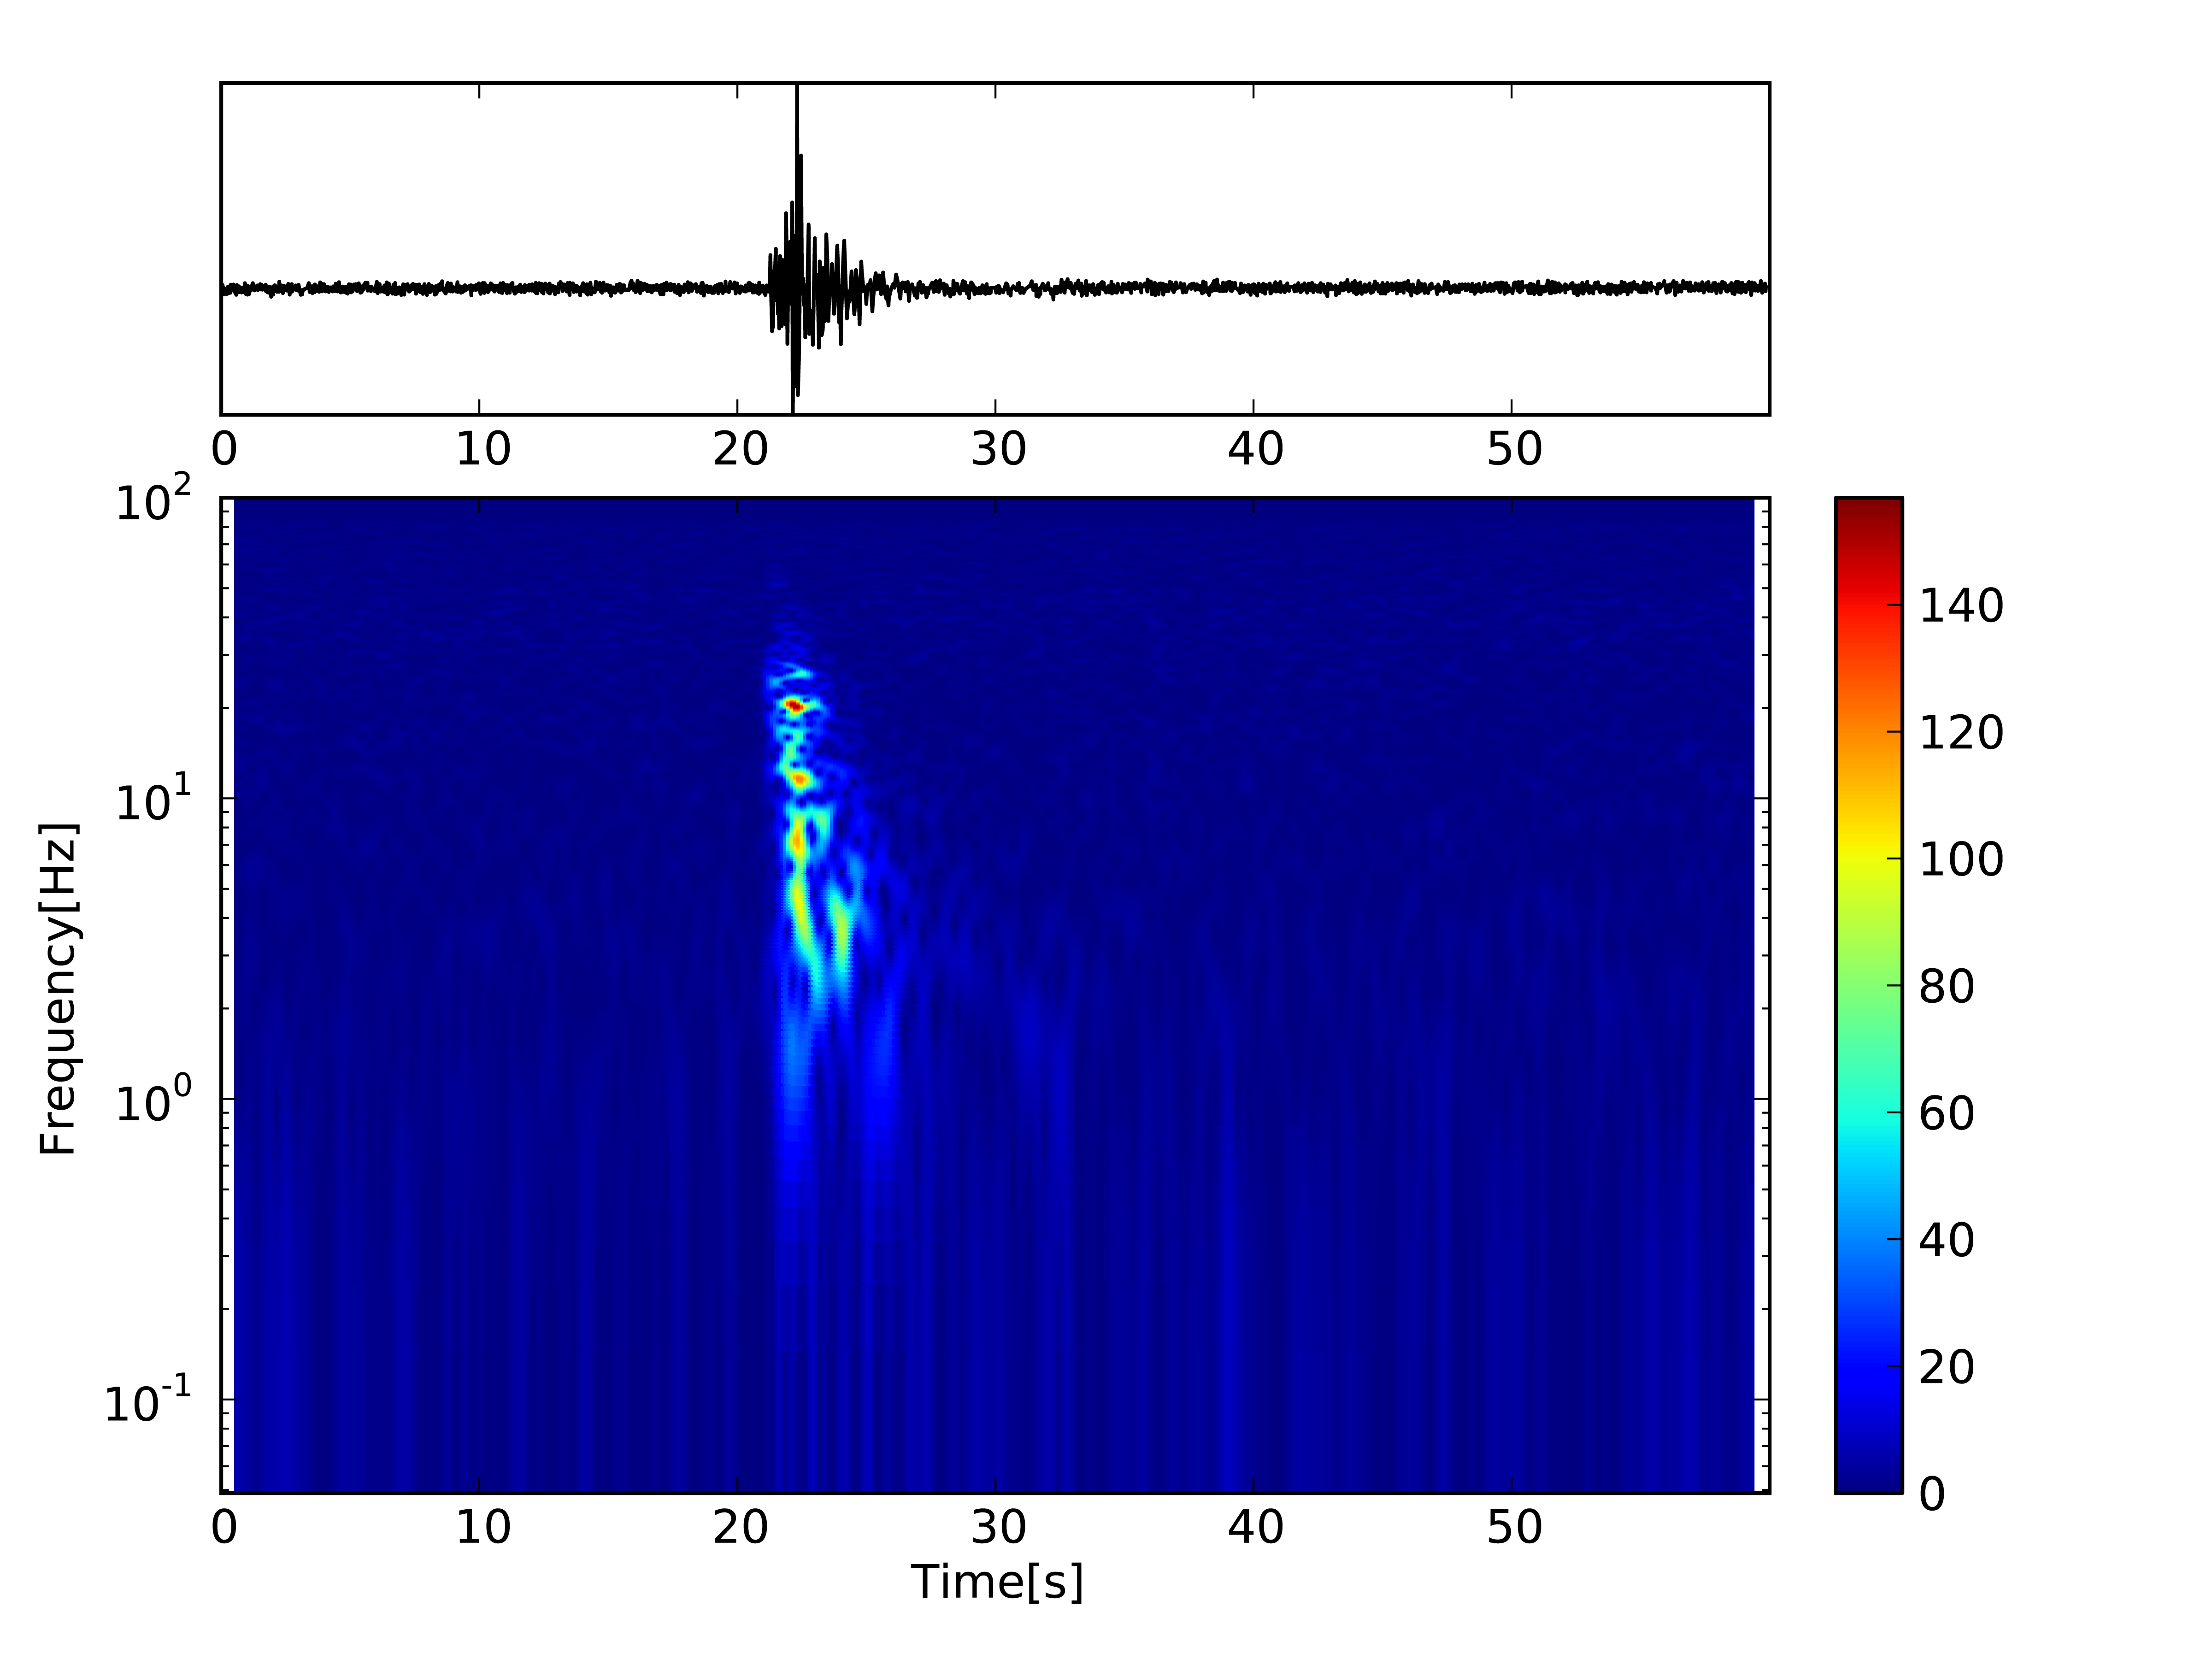
\includegraphics[width=0.45\textwidth]{spectrogram}}
%\end{figure}


%\begin{center}
%\begin{minipage}{\textwidth}
%\begin{center}
%%
%%\begin{minipage}{0.35\textwidth}
%\fbox{
%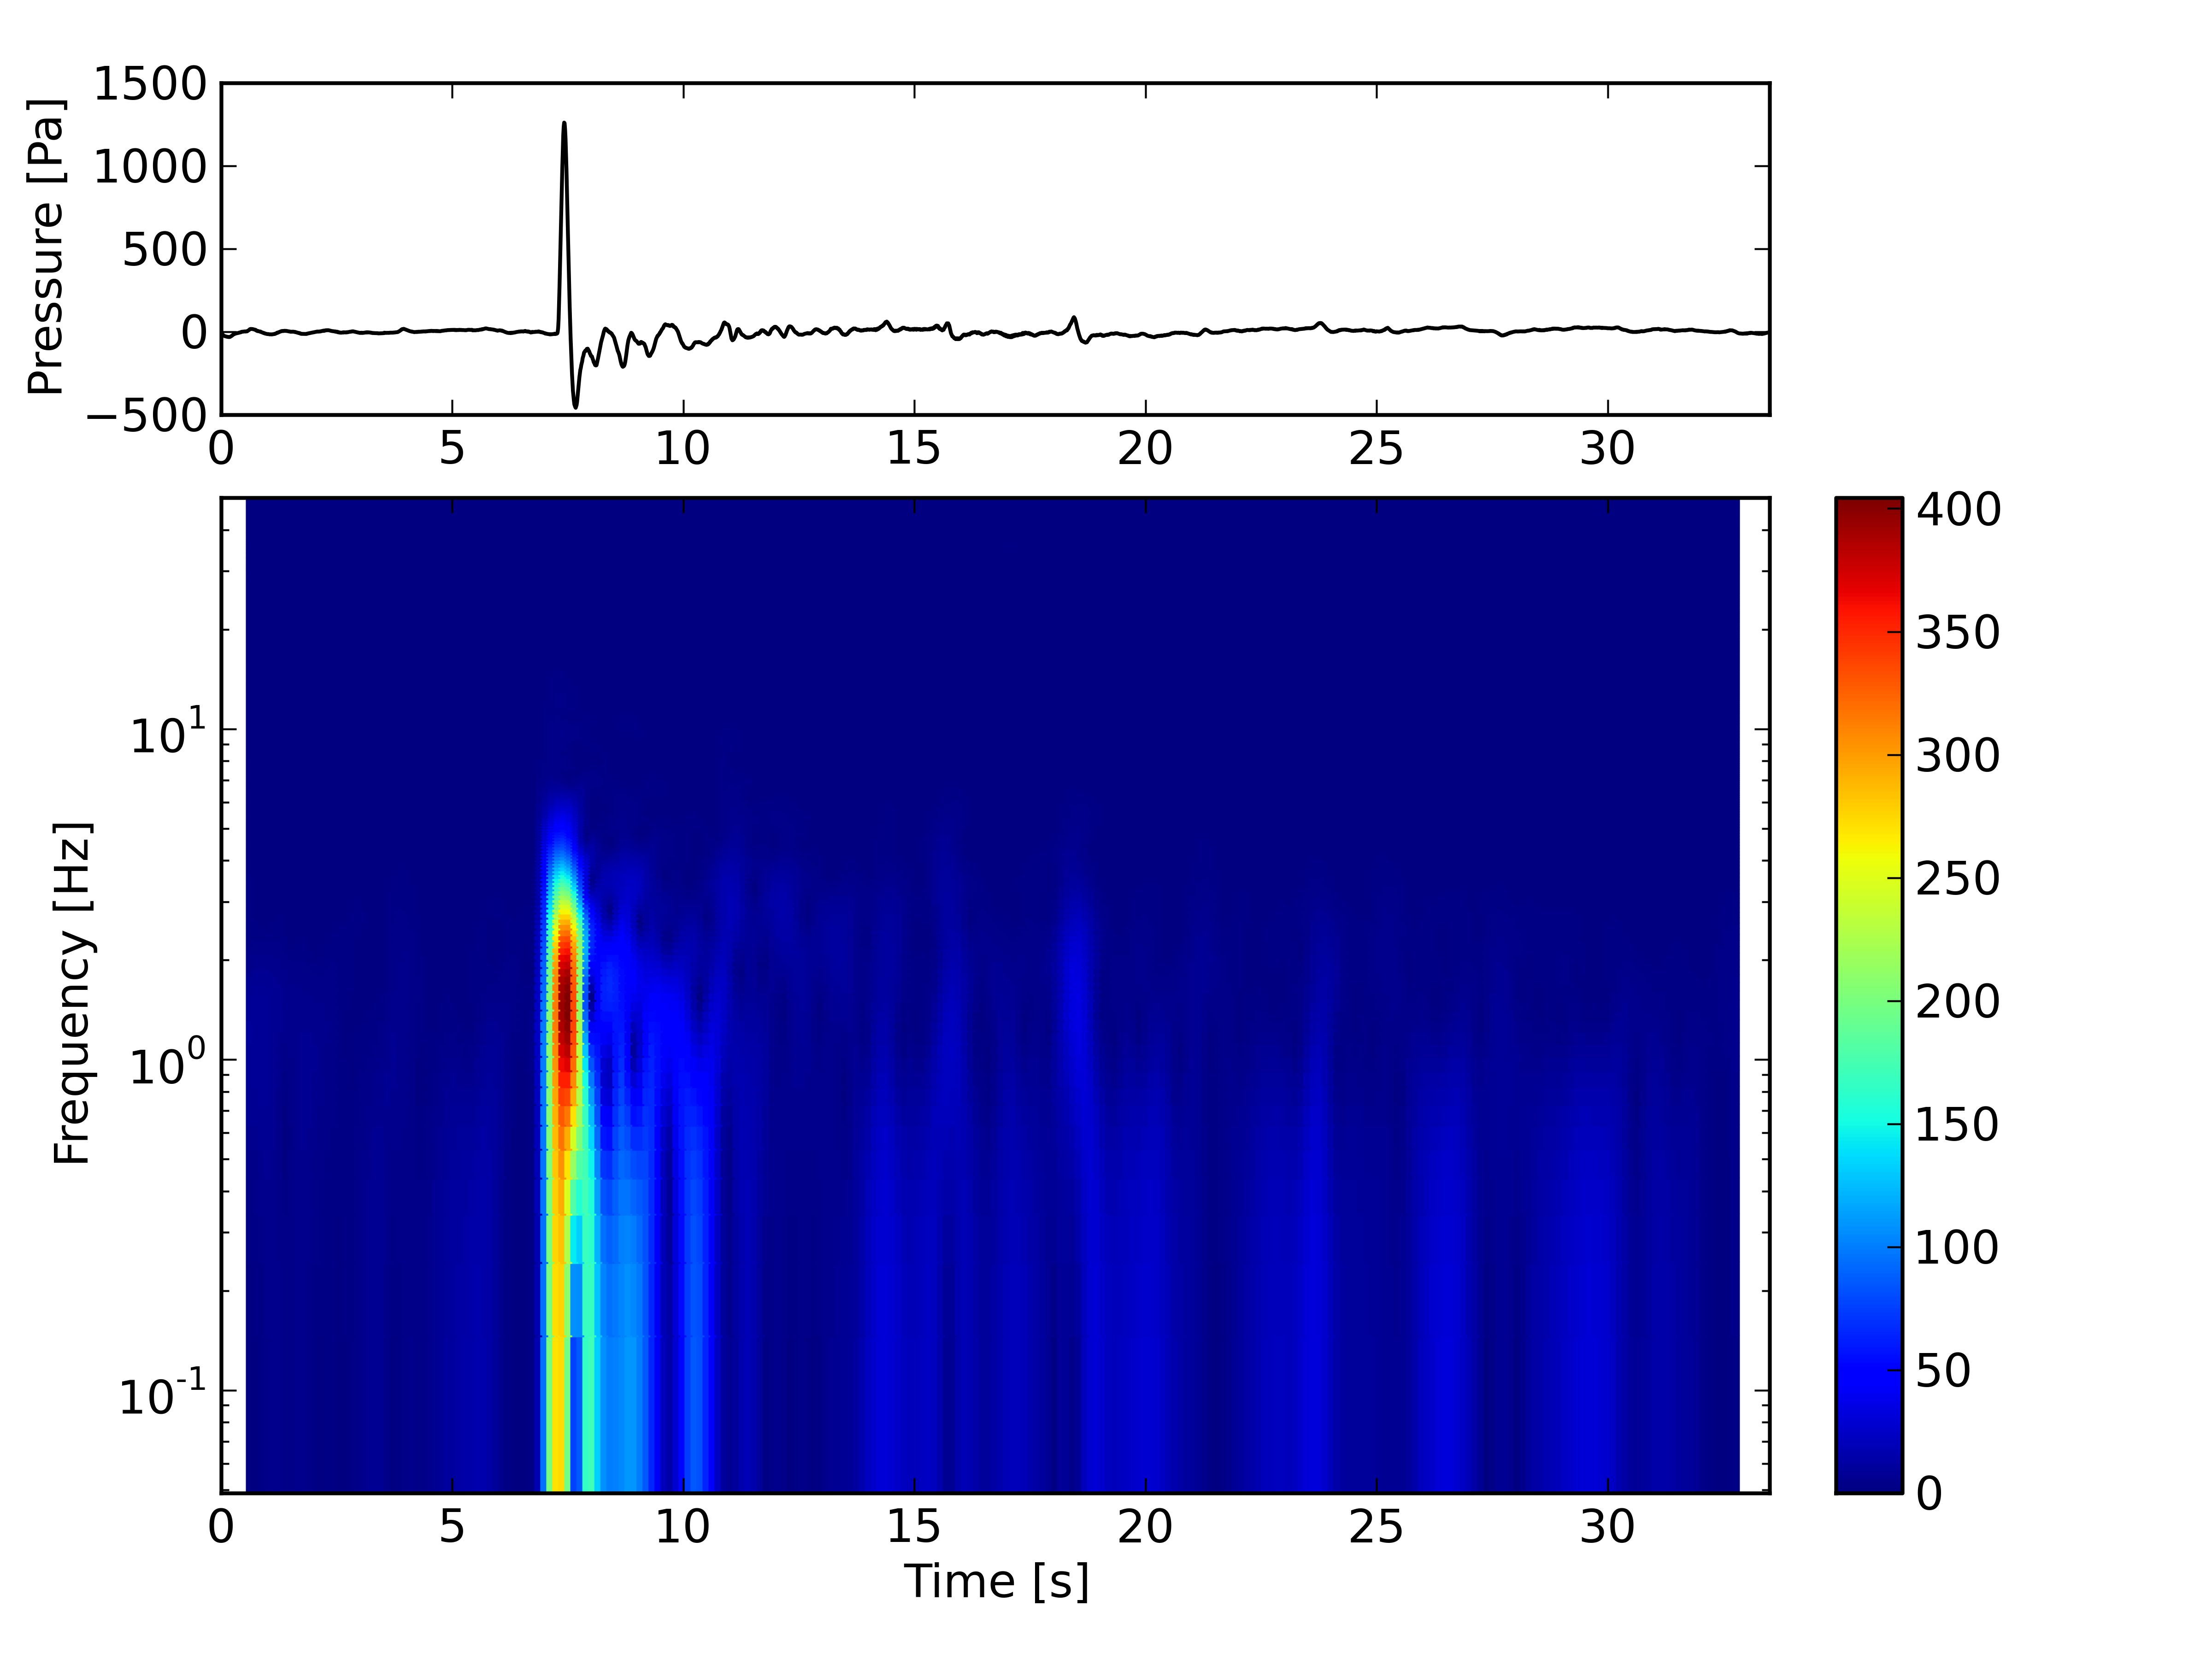
\includegraphics[height=0.35\textwidth]{spectrogram_small}
%}
%%\captionof{figure}{Ein Mithilfe von obspy.imaging.spectrogram erzeugtes Spectrogramm.}
%\hspace{4ex}
%%\end{minipage}
%%
%%\begin{minipage}{0.35\textwidth}
%\fbox{
%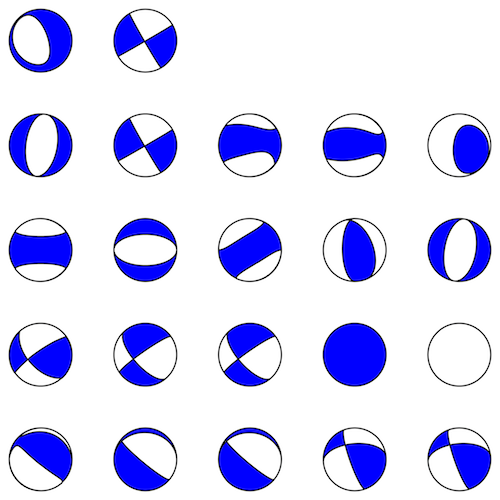
\includegraphics[height=0.35\textwidth]{beachballs_small}
%}
%%\end{minipage}
%
%%\end{center}
%%\end{minipage}
%\end{center}
}\vspace{\MyBoxVSep}
\MyBox[8em]{
\section*{8~~~http://www.obspy.org, weitere Informationen}
Auf der Homepage des Projekts \textbf{http://www.obspy.org} befindet sich eine ausführliche \textbf{Dokumentation}, ein Tutorial, Installationsanleitungen für mehrere Platformen, zahlreiche Beispiele und viele weitere Hinweise, die den Einstieg in ObsPy erleichtern.
\newline
Mehrere Entwickler verschiedenster Institutionen beteiligen sich an ObsPy und sind auf der Homepage offen für Vorschläge, Anregungen und Kritik.
\newline

\underline{\textbf{Weitere Funktionen von ObsPy}}
\begin{itemize}
\item \textbf{obspy.signal:} Filtern, Triggern, Rotieren, Magnitudenbestimmung, Instrumentenkorrektur, Koordinatentransformationen
\item \textbf{obspy.arclink, obspy.fissures, obspy.seishub:} Datenaquisation von \textbf{ArcLink/WebDC}, \textbf{IRIS DMC DHI/Fissures} und \textbf{SeisHub} (www.seishub.org) \citep{seishub}.
\end{itemize}

%Das \textbf{obspy.signal} Modul kann Filtern, Triggern, Rotieren und sowohl Instrumentenkorrekturen als auch Koordiantentransformationen durchführen.
%\newline
%Zudem ist Obspy in der Lage mit Hilfe der Module \textbf{obspy.seishub}, \textbf{obspy.arclink} und \textbf{obspy.fissures} Daten von \textbf{SeisHub}, \textbf{ArcLink/WebDC} und \textbf{IRIS DMC DHI/Fissures} anzufordern.
}\vspace{\MyBoxVSep}

%
% Ninth box.
%
\MyBox[8em]{
\section*{9~~~Literatur}
\bibliography{poster}{}
\bibliographystyle{plaindin}
}\vspace{\MyBoxVSep}

\end{multicols}
% First reduce the vertical spacing to zero and then expand again.
\vspace{-0.60cm}
\vspace{\MyBoxVSep}

% New width.
\setlength{\MyBoxWidth}{736.5mm}
% Single Large Box to take care of the example.
\MyBox[8em]{
\begin{multicols}{3}
\section*{5~~~obspy.imaging (Basemap)}
Diese Anwendung generiert einen topographischen Kartenauschnitt mitsamt Stationen und einigen Herdflächenlösungen.
Dazu werden zunächst via \textbf{obspy.seishub} die Stationsmetadaten in dem Bereich abgefragt und anschließend alle Events im Gebiet.
Die Karte wird mit Hilfe des \textbf{Basemap Toolkits} von \textbf{Matplotlib} dargestellt und die Herdflächenlösungen stammen aus \textbf{obspy.imaging}.

Das gesamte Skript ist einschließlich Kommentare und Leerzeilen nur 80 Zeilen lang.
\subsection*{Codeauschnitte}
Abruf der Stationsmetadaten via obspy.seishub.
\lstinputlisting[firstline=11, lastline=14, firstnumber=11]{code/example.py}
\columnbreak
\begin{center}
\begin{tikzpicture}
\node[above right,text width=.21\MyBoxWidth]at(0cm,0cm){ 
\tiny
\centering
\includegraphics[height=.21\MyBoxWidth]{map}\\[-3ex]
};
\end{tikzpicture}
{\newline \small \textbf{Abbildung~5}: Ausgabe des Skriptes. Es zeigt das Gebiet Hochstaufen. Rote Dreiecke kennzeichnen vorhandene seismische Stationen.
} \\[.5\MyBoxVSep]
\end{center}

\columnbreak
Abruf der Eventdaten.
\lstinputlisting[firstline=21, lastline=23, firstnumber=21]{code/example.py}
Erzeugung der Basemap.
\lstinputlisting[firstline=45, lastline=47, firstnumber=45]{code/example.py}
Zeichnen der Herdflächenlösungen.
\lstinputlisting[firstline=73, lastline=75, firstnumber=73]{code/example.py}
\lstinputlisting[firstline=77, lastline=77, firstnumber=77]{code/example.py}






\end{multicols}
}
\end{document}
